\documentclass[12pt]{article}

\usepackage[utf8]{inputenc}
\usepackage{setspace}
\usepackage[left=2.5cm, right=2.5cm, top=2.5cm, bottom=2.5cm]{geometry}
\usepackage{graphicx}
\usepackage[font=large,labelfont=bf]{caption}
\usepackage{indentfirst}
\usepackage{anyfontsize}
\usepackage{textcomp}

\setlength{\parindent}{5ex}
\graphicspath{}
\renewcommand{\familydefault}{\sfdefault}
\setstretch{1}

\begin{document}
	
\begin{titlepage}
	
\Huge \centering {\sc{\bf{Introduction Homework}}}

\LARGE Geneva Porter, Applied Mathematics

5 September 2018

\vspace{10mm}

\Large \it San Diego State University

Professor J. Mahaffy, Math 636

\end{titlepage}


\section*{\LARGE Chirps and Temperature, Problem 2 (d)}
\normalsize

This problem examines the relationship between ambient temperature and the number of chirps crickets produce in a given time. The graph below (figure 1) shows two theoretical linear models for predicting temperature based on the number of observed cricket chirps per minute. Observational data points are included for both models.

\vspace{0mm}

\begin{figure}[h]
\centerline{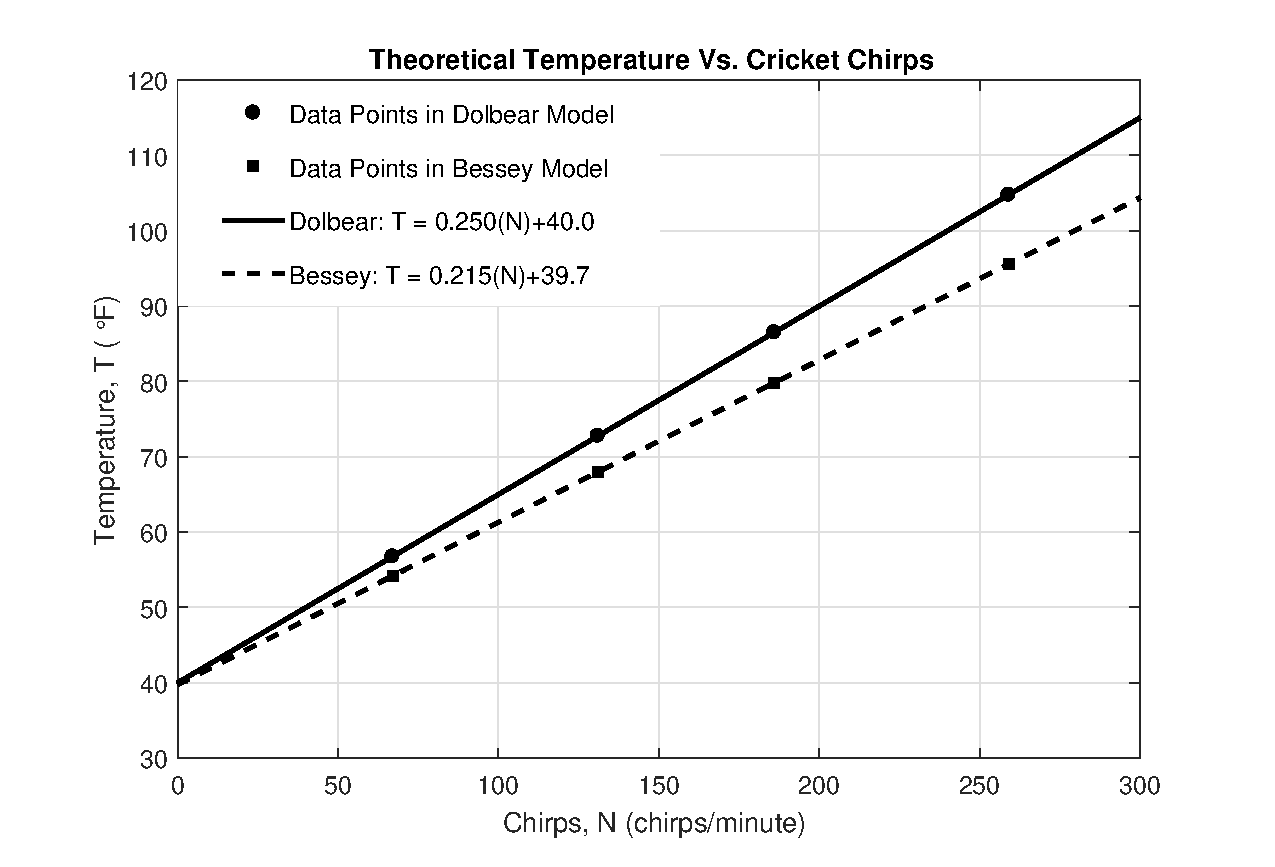
\includegraphics[width=18cm]{HW1PR2.eps}}
\caption{\bf Dolbear and Bessey model comparison}
\end{figure}

\vspace{0mm}

The data points were collected by listening to 4 recordings of crickets chirping over 5 or 6-second intervals,then calculating the number of chirps per minute, or N. These measurements were then matched to the true number of chirps per minute as given in the problem. The data collected both overestimated and underestimated the true number of chirps per minute. For example, the recording of cricket A yielded 7 chirps in 5 seconds, which would be calculated as 84 chirps per minute. However, the true number of chirps per minute was 67. 

Obviously, there were sources of error when collecting data. First, the recordings were only a brief snippet of the cricket's behavior. If the observation period was longer, then the accuracy of the data would improve. Another source of error was the precision of the cricket chirps. The length of a single chirp may vary due to slight fluctuation in temperature, the cricket's own metabolic changes, or an anomaly in the structure of its wings. Obviously, there is also the possibility of human error regarding data collection and analysis.

We can see from the graph that the difference between the two models increases with temperature. The Dolbear model is a simplification of the relationship between chirps and temperature, and it has been used as a "folk method" for at least the last 100 years. Clearly, the Dolbear model is not intended to be precise. On the other hand, the Bessey model was formulated based on several observations and created after careful analysis. It is therefore logical that the Bessey model would be more accurate at predicting temperature. From Figure 1 we can see that the Bessey model predicts temperatures lower than the Dolbear model, due to the lower intercept and smaller slope. The data points that were applied to the Bessey model are more likely to be closer the the true temperature.



\section*{\LARGE Urea and Absorbance, Problem 3 (c, f, h)}

\normalsize

In this problem, questions regarding urea concentration in animals were examined. Excretion was measured by taking the urea absorption by spectrophotometer, then calculating the concentration. This investigation uses the data from 10 animals to determine absorbance as a function of urea concentration. The graph below (Figure 2) displays this relationship as well as the data collected.

\begin{figure}[h]
	\centerline{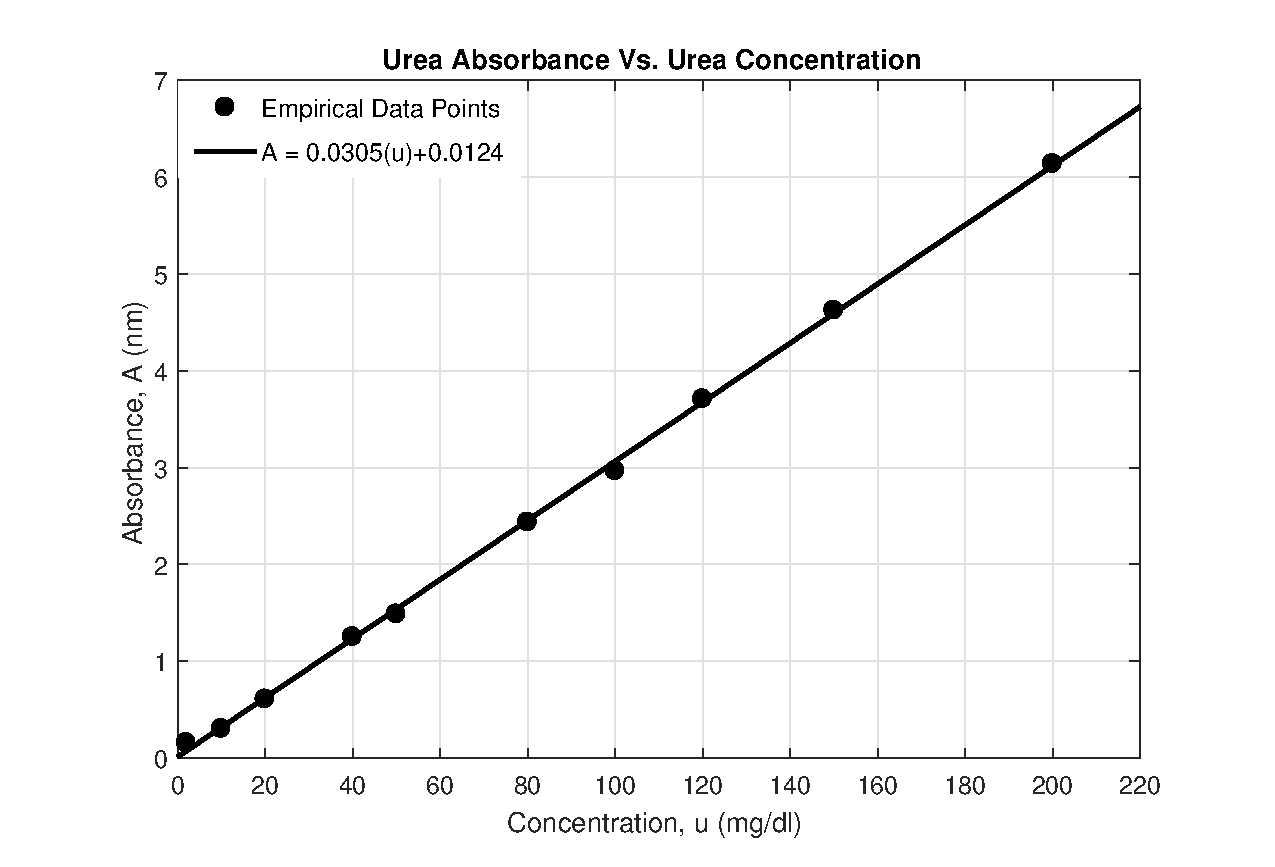
\includegraphics[width=18cm]{HW1PR3.eps}}
	\caption{\bf Dolbear and Bessey model comparison}
\end{figure}

\vspace{0mm}

From this graph, we can see that the linear model fits well, and that urea concentration increases as urea absorption increases. In creating this line, the sum of squared errors was minimized to reduce variance from the model. This error calculation measures the general discrepancy between the data and the values predicted by the model. By slightly changing the slope, the sum of square errors drastically increases. Doubling the slope causes the sum of square errors to increase by several hundred thousand percent. However, doubling the value of the intercept increases the sum of square errors by about six percent.

Another model to consider (not pictured here) is the linear Beer-Lambert model, often used in spectrometry. This model takes to form of:

\centerline{$A = a(\lambda)\cdot b\cdot c$}

Where $A$ is the absorbance, $a(\lambda)$ is the absorptivity coefficient, $b$ is the path length, and $c$ is the analyte concentration (represented by $u$ in Figure 2). The Beer-Lambert model passes through the origin and has a y-intercept of 0. The model shown above has an intercept of $\approx$ 0.01. The difference in these models may be attributed to the narrowness and variance of the data collected. The Beer-Lambert model is a general formula that can be used for a variety of substances, while Figure 2 exclusively maps urea absorption. Also, there were only 10 data points available to create the model, and the intercept may be closer to zero if more data was included in this analysis. 

The concentration of urea in hummingbirds at varying degrees was also calculated. Using the inverse of the model in Figure 2, values of absorbance were input to obtain urea  concentration. Below is a table of the values given:

\vspace{0mm}
\begin{table}[htb]
	\centerline{
	\begin{tabular}{ccc}
	\renewcommand{\arraystretch}{1.5}
		\textit{\textbf{\Large Temperature}}           & \textit{\textbf{\Large Absorbance}} & \textit{\textbf{\Large Concentration}} \\
		\textit{\Large 10\textcelsius }                & \textit{\Large 0.145 nm}            & \textit{\Large 4.34 mg/dl}             \\
		\textit{\Large 20\textcelsius}                 & \textit{\Large 0.201 nm}            & \textit{\Large 6.18 mg/dl}             \\
		\textit{\Large 30\textcelsius}                 & \textit{\Large 0.290 nm}            & \textit{\Large 9.09 mg/dl}              
	\end{tabular}
	}
\end{table}

From these data, we can see that hummingbirds have relatively low levels of urea concentration, and excrete even less urea per mg at colder temperatures. Producing uric acid uses little water, but takes more energy. Conversely, high volumes of water are needed to prevent toxicity from urea (or ammonia) when creating it, but takes less energy. It is possible that, in colder temperatures, hummingbirds have a greater need for water, thus diluting the concentration of urea. In warmer weather, urea concentrations rise, which indicates water consumption may be slightly less than in colder weather. In either case, hummingbirds still need a moisture-rich diet in water to survive. In addition, hummingbirds have an extremely high metabolic rate, and constantly need to conserve energy. This indicates that they would not produce much uric acid to excrete waste.

These conjectures apply to hummingbirds in an active state. In the evening, hummingbirds go into a state of {\it topor}, a deep sleep that slows their metabolic rate and greatly reduces their energy expenditure. During this time it may be more likely that hummingbirds produce close to zero uric acid as a strategy to conserve energy. This would imply that they either loose hydration during {\it topor} by using water to create urea or ammonia, or don't excrete any waste at all. This may be another reason why hummingbirds need a water-rich diet.

Interestingly, a frog's urea excretion pattern is much like the hummingbird's. Also like hummingbirds, frogs have high metabolic rates and need an abundance of water to survive. Since frogs easily intake water through their skin, their bodies favor using more water to excrete waste. Many species of frog also enter states of {\it torpor}, often to survive freezing temperatures. These similarities indicate that frogs may also excrete more urea and need more water at higher temperatures, as well as when in {\it torpor}. Below is a table that gives absorbance rates of a few other animals:

\vspace{0mm}
\begin{table}[htb]
	\centerline{
		\begin{tabular}{ll}
			\renewcommand{\arraystretch}{1.5}
			\textit{\textbf{\Large Animal}}           & \textit{\textbf{\Large Absorbance}} \\
			\textit{\Large  Chicken }             & \textit{\Large 3.19 nm}       \\
			\textit{\Large  Duck (fresh water)}                 & \textit{\Large 0.452 nm}       \\
			\textit{\Large  Duck (salt water)}                 & \textit{\Large 0.790 nm}       \\       
			\textit{\Large  Frog}                 & \textit{\Large 0.262 nm}       \\ 
			\textit{\Large  Turtle}                 & \textit{\Large 1.09 nm}       \\ 
			\textit{\Large  Tortoise}                 & \textit{\Large 6.80 nm}       
		\end{tabular}
	}
\end{table}

Looking at absorbance rates for other animals, there is a correlation between animals with high metabolic rates and low urea concentration. Both species of duck have urea concentrations below one, which correlates to the high metabolic rate needed for migratory aviation and the necessity to conserve energy while having easy access to water during such migrations. We also see that the chicken and tortoise have urea concentrations higher than one. These animals typically have lower metabolic rates and process waste much more slowly. They may also have more need to conserve water in their habitats, therefore the urea they do produce is more heavily concentrated. In general, it seems that low urea concentrations appear in animals with high metabolic rates with easy access to water.

\section*{\LARGE Pulses and Temperature, Problem 4 (h)}

\normalsize

Revisiting the correlation between crickets and temperature, this problems examines the stridulation process that produces the rapid pulses that compose a cricket's chirp. Figure 3 (next page) displays several best-fit lines that describe the pulse rate of a chirp in relation to temperature.

Figure 3 displays 3 models from observational data points on temperature vs. cricket pulses per second. A linear, quadratic, and cubic best fit are shown. For temperatures between 70 and 95 degrees Fahrenheit, all three models fit the data with similar accuracy. The sum of squared errors suggests that accuracy improves as the degree of the polynomial increases. The sum of squared errors for the linear and quadric models are similar, with a slight improvement (that is, a smaller value) for the quadratic model. The cubic model shows a more significant decrease in the sum of squared errors. Conversely, Looking at the BIC and AIC of these models suggests that the linear model is the most accurate and the cubic is the least accurate for both cases. For temperatures outside this range, the cubic model would likely be highly inaccurate. More data would be needed to determine if the linear or quadratic model is more accurate outside this range.

As with nearly any mathematical model, this one can be improved. The most obvious improvement would be an increase in data points, which would alter the parameters of the models and hopefully provide better predictive power. Along this line, obtaining data outside the range of 70 to 95 degrees Fahrenheit would yield an improved general model.  
\pagebreak
\begin{figure}[h]
	\centering{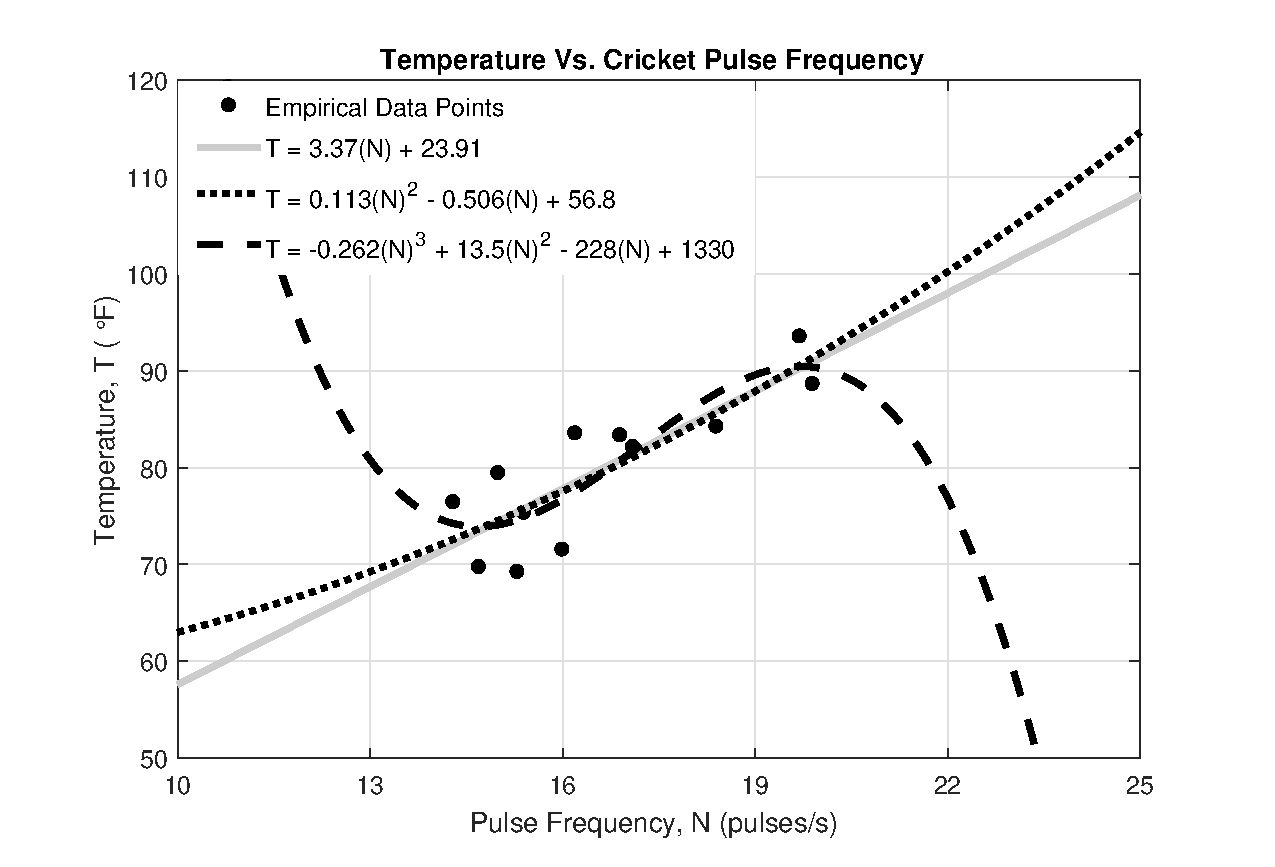
\includegraphics[width=18cm]{HW1PR4.eps}}
	\caption{\bf Dolbear and Bessey model comparison}
\end{figure}
\end{document}




























